\PassOptionsToPackage{unicode=true}{hyperref} % options for packages loaded elsewhere
\PassOptionsToPackage{hyphens}{url}
%
\documentclass[]{article}
\usepackage{lmodern}
\usepackage{amssymb,amsmath}
\usepackage{ifxetex,ifluatex}
\usepackage{fixltx2e} % provides \textsubscript
\ifnum 0\ifxetex 1\fi\ifluatex 1\fi=0 % if pdftex
  \usepackage[T1]{fontenc}
  \usepackage[utf8]{inputenc}
  \usepackage{textcomp} % provides euro and other symbols
\else % if luatex or xelatex
  \usepackage{unicode-math}
  \defaultfontfeatures{Ligatures=TeX,Scale=MatchLowercase}
\fi
% use upquote if available, for straight quotes in verbatim environments
\IfFileExists{upquote.sty}{\usepackage{upquote}}{}
% use microtype if available
\IfFileExists{microtype.sty}{%
\usepackage[]{microtype}
\UseMicrotypeSet[protrusion]{basicmath} % disable protrusion for tt fonts
}{}
\IfFileExists{parskip.sty}{%
\usepackage{parskip}
}{% else
\setlength{\parindent}{0pt}
\setlength{\parskip}{6pt plus 2pt minus 1pt}
}
\usepackage{hyperref}
\hypersetup{
            pdfborder={0 0 0},
            breaklinks=true}
\urlstyle{same}  % don't use monospace font for urls
\usepackage{graphicx,grffile}
\makeatletter
\def\maxwidth{\ifdim\Gin@nat@width>\linewidth\linewidth\else\Gin@nat@width\fi}
\def\maxheight{\ifdim\Gin@nat@height>\textheight\textheight\else\Gin@nat@height\fi}
\makeatother
% Scale images if necessary, so that they will not overflow the page
% margins by default, and it is still possible to overwrite the defaults
% using explicit options in \includegraphics[width, height, ...]{}
\setkeys{Gin}{width=\maxwidth,height=\maxheight,keepaspectratio}
\setlength{\emergencystretch}{3em}  % prevent overfull lines
\providecommand{\tightlist}{%
  \setlength{\itemsep}{0pt}\setlength{\parskip}{0pt}}
\setcounter{secnumdepth}{0}
% Redefines (sub)paragraphs to behave more like sections
\ifx\paragraph\undefined\else
\let\oldparagraph\paragraph
\renewcommand{\paragraph}[1]{\oldparagraph{#1}\mbox{}}
\fi
\ifx\subparagraph\undefined\else
\let\oldsubparagraph\subparagraph
\renewcommand{\subparagraph}[1]{\oldsubparagraph{#1}\mbox{}}
\fi

% set default figure placement to htbp
\makeatletter
\def\fps@figure{htbp}
\makeatother


\date{}

\begin{document}

\hypertarget{scientific-practice}{%
\section{Scientific practice}\label{scientific-practice}}

\hypertarget{solutions}{%
\subsection{solutions}\label{solutions}}

\hypertarget{electrolytic-solutions}{%
\subsubsection{electrolytic solutions}\label{electrolytic-solutions}}

Ionic dissociation occurs when the addition of a solvent or energy in
the form of heat causes molecules if crystals of a substance to break
down into ions.

\hypertarget{osmotic-effects.}{%
\subsubsection{Osmotic effects.}\label{osmotic-effects.}}

spontaneous net movement of solvent molecules through a semipermeable
membrane

\hypertarget{tonicity}{%
\subsubsection{tonicity}\label{tonicity}}

\hypertarget{hypotonic}{%
\paragraph{hypotonic}\label{hypotonic}}

lower ions concentration, high solvent concentration lower osmotic
pressure

\hypertarget{hypertonic}{%
\paragraph{hypertonic}\label{hypertonic}}

higher ion concentration, higher solute concentration, lower solvent
concentration, higher osmotic pressure

\hypertarget{isotonic}{%
\paragraph{isotonic}\label{isotonic}}

equal osmotic pressure. and solute/solvent concentrations.

\hypertarget{ideal-solutions}{%
\subsubsection{Ideal Solutions}\label{ideal-solutions}}

an ideal solution is a solution which has a enthalpy of solution equal
to zero NOTE: bonds forming releases heat energy. FR: the concentration
of water in a typical cell is 55molar.

\hypertarget{concentration-measurements}{%
\subsubsection{concentration
measurements}\label{concentration-measurements}}

\hypertarget{molarmolaritymolar-concentration}{%
\paragraph{molar/molarity/molar
concentration}\label{molarmolaritymolar-concentration}}

concentration of solute in a solution in terms of moles of solute per
volume of solution

\hypertarget{molality}{%
\paragraph{molality}\label{molality}}

concentration of solute in a solution in terms of moles of solute per
mass of solvent.

\hypertarget{other-measures.}{%
\paragraph{Other measures.}\label{other-measures.}}

\%w/w weight of solute per weight of (solvent?)

\%w/v weight per volume.

\%v/v volume per volume.

\hypertarget{osmolarity}{%
\paragraph{osmolarity}\label{osmolarity}}

concentration of solute as total number of solute particles per litre
(?)

\hypertarget{osmolality}{%
\paragraph{osmolality}\label{osmolality}}

Concentration of solute as total number of solute particles per
kilogram.

\#\#\#\#osmol number of solute particles which contribute towards the
osmolarity of the substance.

\#\#Life Molecules

\hypertarget{basic-list}{%
\subsubsection{Basic list}\label{basic-list}}

\begin{itemize}
\tightlist
\item
  Carbohydrates (2\%)
\item
  Lipids (2.5\%)
\item
  Proteins (15\%)
\item
  Nucleic Acids (RNA 20\% E. Coli \textless{} 10\% mammalian DNA is
  functional )
\item
  Inorganic ions (3\% Salts, 1\% small metabolites)
\item
  water (70\%)
\end{itemize}

\hypertarget{water}{%
\subsubsection{Water}\label{water}}

\hypertarget{general-properties}{%
\paragraph{general properties}\label{general-properties}}

covalent bonds. dipole moment.

\hypertarget{hydrogen-bonds.}{%
\subparagraph{hydrogen bonds.}\label{hydrogen-bonds.}}

many hydrogen bonds are formed which together gain considerable
strength.

Hydrogen bonds are typically up to \$ angstroms in length, which a
strength of 2-10kcal/mol.

NOTE: the advantage of hydrogen bonds is that they do not take too much
energy to break down so the body can readily re-purpose/recycle organic
compounds.

\hypertarget{polarity}{%
\subparagraph{polarity}\label{polarity}}

high polarity means water has a large ability to stabilise other charges

\hypertarget{section}{%
\subparagraph{}\label{section}}

auto ionisation. water can auto ionise into hydroxide ions and hydronium
ions, the concetrations of which in solution can be measured by pOH and
pH respectively.

\hypertarget{solvation-of-ionic-and-polar-solutes}{%
\subparagraph{Solvation of ionic and polar
solutes}\label{solvation-of-ionic-and-polar-solutes}}

\(Coulomb’s\ law: F = k\frac{ q_{1}q_{2}}{ Dr^{2}}\)

Where D is a measure of solvent polarity.The higher the polarity, the
greater the ability to stabilise charges. water forms solvations shells
around each ion.

\hypertarget{solvation-of-apolar-groups-and-molecules-the-hydrophobic-effect}{%
\subparagraph{Solvation of apolar groups and molecules (the hydrophobic
effect)}\label{solvation-of-apolar-groups-and-molecules-the-hydrophobic-effect}}

free amphipathic molecules will associate in water to form hydrophobic
internal environments. molecules (amphipathic molecules contain both
polar and a polar groups )

Examples

Integral proteins within the cell membrane are amphipathic, and allow
for non polar channels through the membrane.

fatty acids form micelles (globules) and bilayers in water.

\begin{figure}
\centering
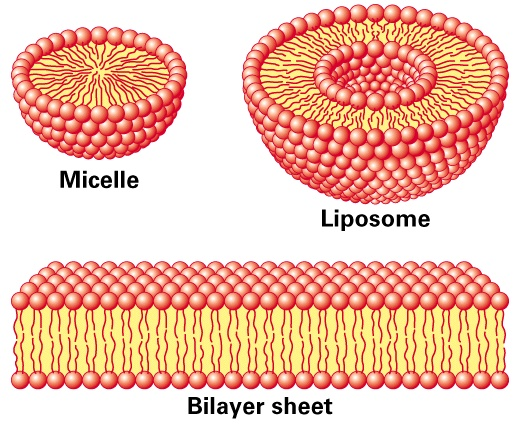
\includegraphics[width=0.5\textwidth,height=\textheight]{Images/FattyAcidsInWater.JPG}
\caption{hydrophobicEffect}
\end{figure}

Septicaemia

Certain bacteria, respond to antibiotics by releasing proteins which
punch holes in the cell surface membrane creating freely permeable pore
through which cell contense can leak out, and killing the cells.

\hypertarget{water-and-protein-structure}{%
\paragraph{water and protein
structure}\label{water-and-protein-structure}}

water proteins can be buried in the interior of protein structures where
they may furfill vital functions

\hypertarget{examples-1}{%
\subparagraph{examples}\label{examples-1}}

proteases only work if the have a water molecule imbedded within their
internal structure, without this one molecule the entire enzyme becomes
inactive.

other examples are reverse transcriptase and HIV protease and GST
(detoxifying enzyme) which all rely on water molecules to function.

\hypertarget{acids-and-bases}{%
\subsection{Acids and Bases}\label{acids-and-bases}}

\hypertarget{bronsted-and-lowery}{%
\subsubsection{Bronsted and lowery}\label{bronsted-and-lowery}}

acids are proton donors bases are proton acceptors. difference between
acid/base and its conjugate is a proton.

\hypertarget{lewis}{%
\subsubsection{lewis}\label{lewis}}

acids are electron pair acceptors bases are electron pair donors.

\hypertarget{lewis-bases}{%
\paragraph{lewis bases}\label{lewis-bases}}

\begin{itemize}
\tightlist
\item
  alchohol
\item
  organophosphates.
\end{itemize}

\hypertarget{buffering}{%
\subsubsection{buffering}\label{buffering}}

relies on weak acids or bases which do nto fully dissociate.

\hypertarget{scientific-reasoning}{%
\section{Scientific Reasoning}\label{scientific-reasoning}}

\hypertarget{basic-structures-of-an-argument}{%
\subsection{Basic structures of an
argument}\label{basic-structures-of-an-argument}}

\hypertarget{premises}{%
\subsubsection{Premises}\label{premises}}

A Premise is a statment. This statement may be true or false.

In science the orginial premise is known as the hypothesis. this
hypothesis will be tested, usually impirically.

\hypertarget{conclusions}{%
\subsubsection{Conclusions}\label{conclusions}}

A conclusion should be well supported by all premises. The conclusion
leads one to decide if the hypothesis is true fo false.

\hypertarget{a-good-argument}{%
\subsection{A good argument}\label{a-good-argument}}

A good argument can be deductively, or nondecuctive but abductively, or
inductively strong.

NOTE: Arguments can be invalid even if all of the premises and the
conclusion are true. If they do not actually imply eachother then it is
simply a collection of facts and not an argument.

\hypertarget{deductive-arguments}{%
\subsubsection{Deductive arguments}\label{deductive-arguments}}

\(A \in B \wedge B \in C \rightarrow C \in B\)

\hypertarget{conditional}{%
\paragraph{Conditional}\label{conditional}}

\(\exists P \rightarrow \exists Q\)

\hypertarget{contrapositive}{%
\paragraph{Contrapositive}\label{contrapositive}}

\(\nexists P \rightarrow \nexists Q\)

\hypertarget{converse}{%
\paragraph{Converse}\label{converse}}

\(\exists Q \rightarrow \, \exists P\)

\hypertarget{deductive-validity}{%
\paragraph{deductive validity}\label{deductive-validity}}

\begin{enumerate}
\def\labelenumi{\arabic{enumi}.}
\tightlist
\item
  Are the premices true (this is difficult if not impossible to
  establish in mathematics. )
\item
  Do the premices guarentee the truth on the conclusion.
\item
  does the argument beg the question (Not really one of the criteria)
\end{enumerate}

\hypertarget{non-deductive-arguments}{%
\subsubsection{Non deductive arguments}\label{non-deductive-arguments}}

most of science is actually non deductive reasoning. science will often
venture conclusions beyond the scope of observation (induction).

\hypertarget{inductive-reasoning}{%
\paragraph{Inductive Reasoning}\label{inductive-reasoning}}

In Inductive reasoning premises are veiw as strong support of the truth
of the conclusion. however they do not garuntee the truth of the
conclusion. Induction allows for conclusions to be made about issues
outside the scope of ovservation.

\hypertarget{inductive-strength}{%
\subparagraph{Inductive strength}\label{inductive-strength}}

two factor influence the inductive strength of an argument, sample size
and bias.

\hypertarget{deductive-arguments-1}{%
\subsubsection{Deductive arguments}\label{deductive-arguments-1}}

\hypertarget{abduction}{%
\subsubsection{Abduction}\label{abduction}}

abductive arguments seek to explain what is observed, otherwise known as
inference to best explination.

\hypertarget{abductive-arguments}{%
\paragraph{Abductive arguments}\label{abductive-arguments}}

abductive hypothesies should be able to predict easily testable results,
such that if the predicted result is achieved during experimentation
then the validity of the hypothesis is supported, and if it is not the
hypothesis can be rejected.

(Abductive arguments usually rely on a number of assumptions which can
be supported by the predictive power of the argument)

NOTE: if testing two alternative theories H1 and H0 then a good test
experiment will be set up such that the the observation of event P
supports H0 and negates H1 and visa versa.

\hypertarget{evaluating-abductive-inferences.}{%
\paragraph{Evaluating Abductive
Inferences.}\label{evaluating-abductive-inferences.}}

\hypertarget{surprise-principles}{%
\subparagraph{Surprise principles}\label{surprise-principles}}

If an observation supports a hypothesis, then it must strongly favour
that hypothesis over others with which it competes

In order to satisfy this principle: 1. the hypothesis should make no
fasle predictions 2. Within the set of true predictions which the
hypothesis makes, there should be predictions which are expected NOT to
come true if the hypothesis is false (Is this not mixed up somewhere?)

\hypertarget{abductive-fallacy}{%
\subparagraph{Abductive fallacy}\label{abductive-fallacy}}

A widely used and accepted expination is not necessary at all plausible,
(even if no competing explination exists)

\hypertarget{making-observations}{%
\subsubsection{Making observations}\label{making-observations}}

obervations can be made by human senses as well as by sophisticated
scientific equipment.

\hypertarget{examples-2}{%
\paragraph{examples}\label{examples-2}}

\hypertarget{medelian-genetics.}{%
\subparagraph{Medelian genetics.}\label{medelian-genetics.}}

mendal made conclusions very far beyond his premises, abducting from
color change to the existance and role of gentic elements.

\hypertarget{a-bad-argument}{%
\subsection{A bad argument}\label{a-bad-argument}}

\hypertarget{circular-arguments.}{%
\subsubsection{Circular arguments.}\label{circular-arguments.}}

\(A \in B \rightarrow A \in B\)

\hypertarget{definitions}{%
\section{Definitions}\label{definitions}}

\hypertarget{premise}{%
\subsubsection{Premise}\label{premise}}

A Premise is a statment. This statement may be true or false.

\hypertarget{conclusion}{%
\subsubsection{Conclusion}\label{conclusion}}

\hypertarget{bias}{%
\subsubsection{Bias}\label{bias}}

factors which may skew the results of a test in some form.

\hypertarget{steriochemistry}{%
\section{Steriochemistry}\label{steriochemistry}}

\hypertarget{rotamers}{%
\subsection{Rotamers}\label{rotamers}}

Isomers which can be interconverted by rotation (of a given part of the
molecule) about a particular bond

Different isomers are known as Isoforms.

NOTE: bonds within molecules can lengthed, shorted,bend and rotate,
depending on what stresses are excerted upon them.

\hypertarget{newman-projections}{%
\subsubsection{Newman Projections}\label{newman-projections}}

A visualisation of a moleculeviewed from the front.

the front atom is reprisented as a dot the back atom is reprisented as a
circle.

\hypertarget{conformations}{%
\subsubsection{Conformations}\label{conformations}}

\hypertarget{staggered}{%
\paragraph{Staggered}\label{staggered}}

Surrounding atoms/hydrogens are all equally spaced.

this conformation is more stable for two reasons

\hypertarget{steric-hinderance}{%
\subparagraph{Steric Hinderance}\label{steric-hinderance}}

in the eclipsed conformation outside atoms are forced to close to
eachother, raising the energy level of the conformation

\hypertarget{hyperconjugation}{%
\subparagraph{Hyperconjugation}\label{hyperconjugation}}

stabilising interactions of the electrons in a \(\sigma\)-bond (usually
C-H or C-C) with an adjacent empty or partially filled p-orbital or a
\(pi\)-orbital to give an extended molecular orbital that increases the
stability of the system)

\hypertarget{eclipsed}{%
\paragraph{Eclipsed}\label{eclipsed}}

Outside atoms line up with each other.

NOTE: there are a whole range of conformations depending on the exact
angle of rotation. \href{Images/RotamerEnergyDiagram.jpg}{Rotamer Energy
Diagram}

\end{document}
